\documentclass[12pt]{article}
\usepackage{ctex}
\usepackage{geometry}
\usepackage{graphicx}
\usepackage{subcaption}

\title{ResNet-18与Transformer}
\author{王逸群 19307110397}
\date{2022.5}

\geometry{a4paper,left=2.5cm,right=2.5cm,top=2.5cm,bottom=2.5cm}

\begin{document}
	
\maketitle

GitHub repo 链接:https://github.com/quniLcs/cv-final

网盘链接:

\section{数据集}

本项目使用CIFAR-100数据集,
其中包含60000张$32\times32$的彩色图片,
其中训练集50000张,测试集10000张,
被平均分为100类。

\section{网络结构}

\subsection{ResNet}

本项目使用的第一种网络结构是ResNet-18,
其中激活函数为ReLU,
最大的特征为残差连接。
后者包括两种单元结构如图\ref{fig:ResNet}所示。

\begin{figure}[h]
	\begin{subfigure}{0.5\textwidth}
	    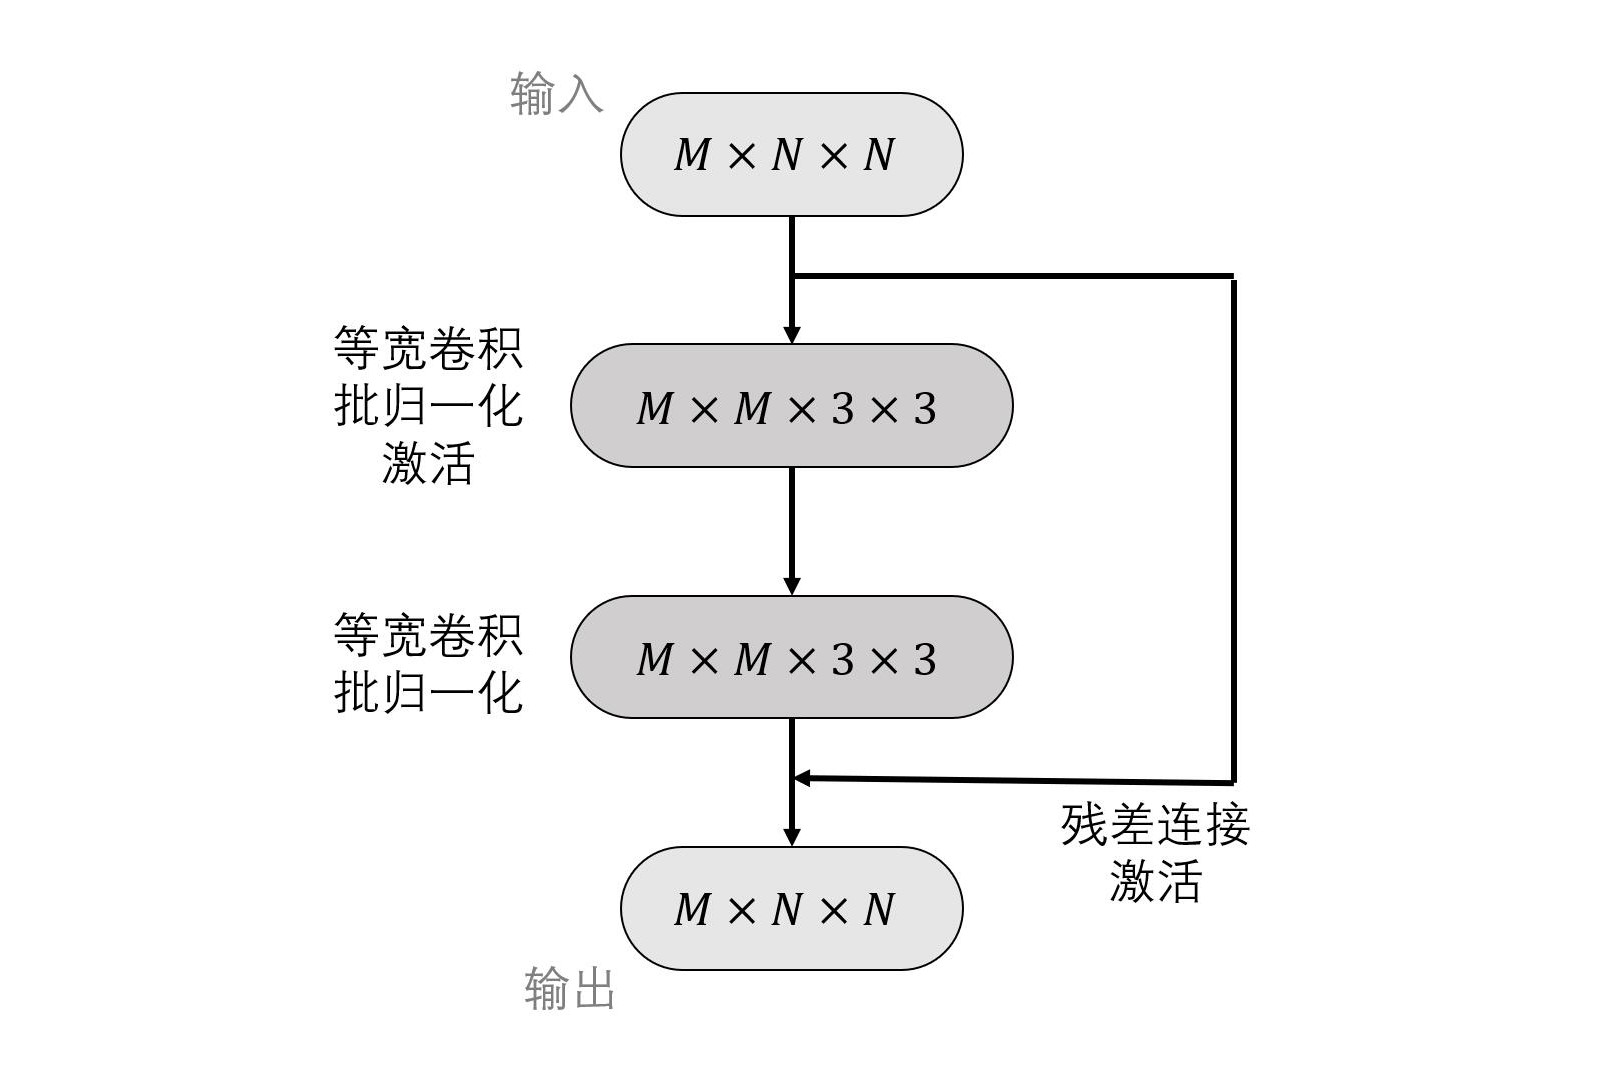
\includegraphics[width=\linewidth]{graph/ResNetI.jpg}
	    \caption{第一种单元结构}
    \end{subfigure}
    \begin{subfigure}{0.5\textwidth}
    	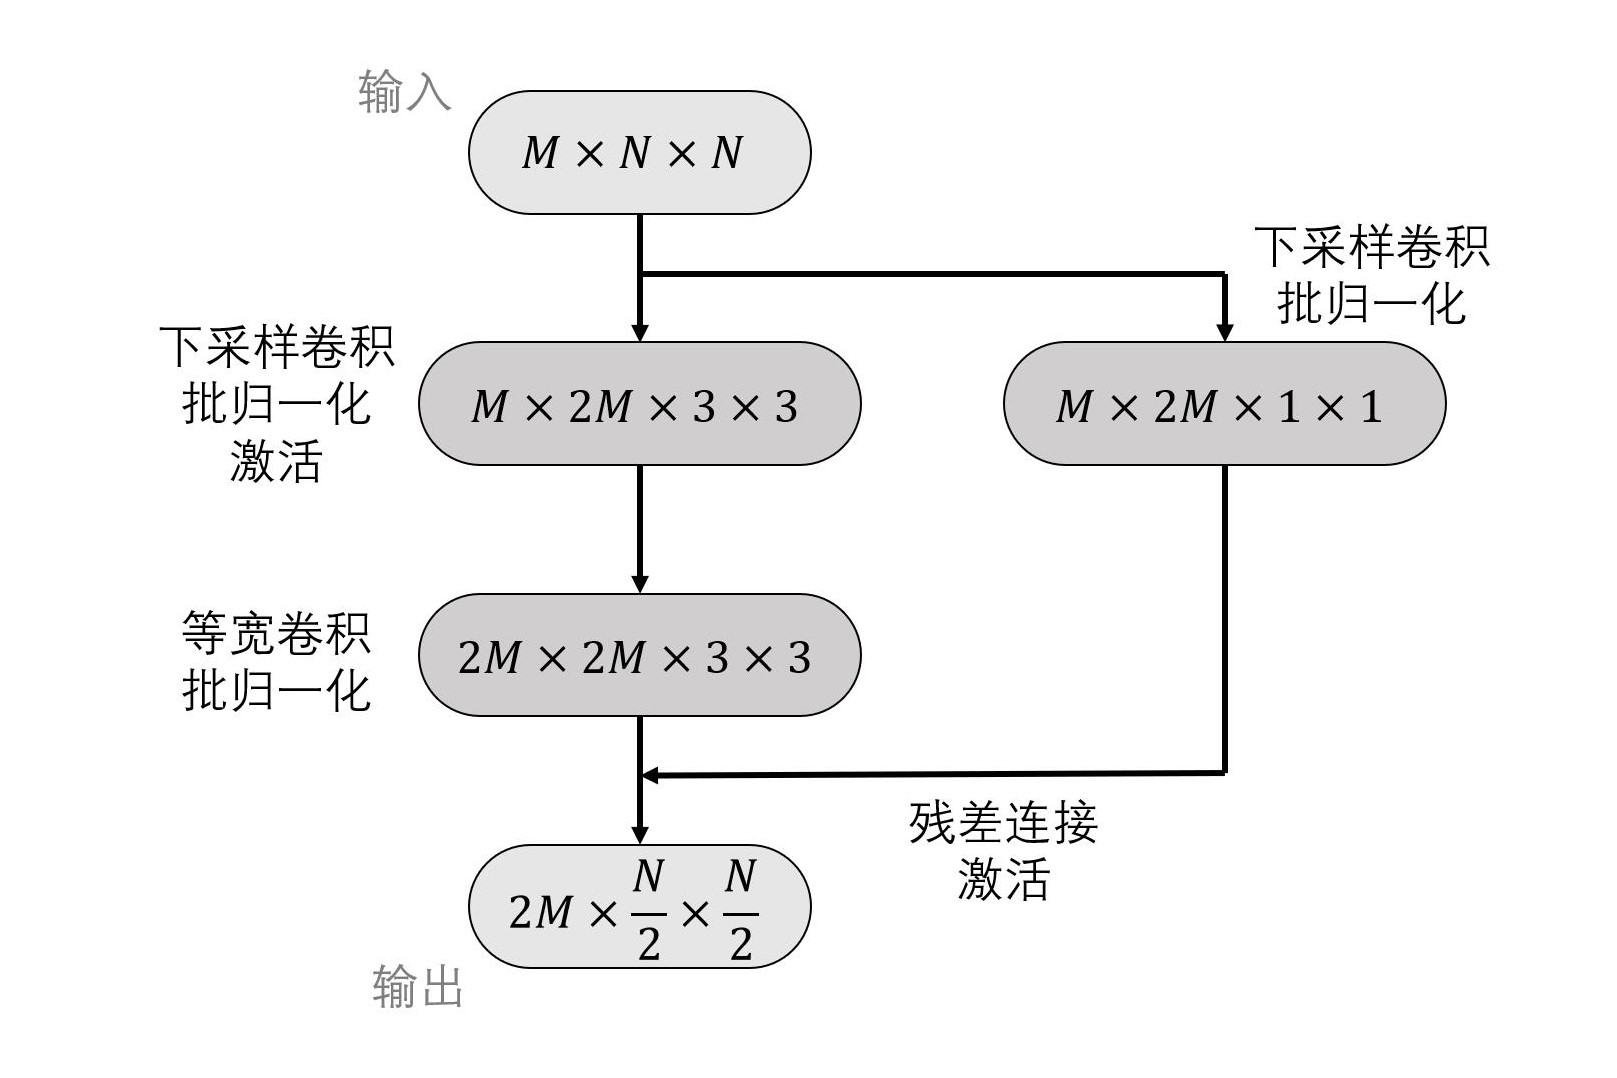
\includegraphics[width=\linewidth]{graph/ResNetII.jpg}
    	\caption{第二种单元结构}
    \end{subfigure}
    \caption{残差连接的两种单元结构}
	\label{fig:ResNet}
\end{figure}

对于输入的图像,
先进行步长为1的$3\times64\times3\times3$卷积操作,
并进行批归一化和激活,
维度变为$64\times32\times32$;
接着通过两次第一种单元结构,维度不变;
再通过第二种单元结构,维度变为$128\times16\times16$;
再通过第一种单元结构,维度不变;
再通过第二种单元结构,维度变为$256\times8\times8$;
再通过第一种单元结构,维度不变;
再通过第二种单元结构,维度变为$512\times4\times4$;
再通过第一种单元结构,维度不变;
最后通过全连接得到输出。
由此,参数数量为11220132.

\subsection{ViT}

本项目使用的第二种网络结构是ViT(Vision Transformer),
其主体是一个Transformer编码器,
其中激活函数为GELU,
如图\ref{fig:ViT}所示。

\begin{figure}[h]
	\includegraphics[width=\linewidth]{paper/ViT.png}
	\caption{ViT网络结构}
	\label{fig:ViT}
\end{figure}

对于输入的图像,
根据给定的 patch size 划分成若干个 patch,
并通过全连接层编码成给定维度的向量,即 patch 编码。
这些 patch 编码和可学习的分类编码
分别与各自的位置编码相加后
进入 Transformer 编码器。
在 Transformer 编码器中,
每个 Transformer 层由
层归一化、多头注意力机制、残差连接、
层归一化、两层前馈神经网络、残差连接所组成。
最后,分类编码对应的 Transformer 编码
通过层归一化和全连接层得到输出。

参考 ViT 原论文、
与 ViT 相关的 Jean-Baptiste Cordonnier 等人的工作、
以及官方开源软件包中模型的默认参数,
选择网络结构参数如表\ref{tab:Transformer}所示。
值得注意的是,
多头注意力机制中隐藏层的总数据维度应与模型隐藏层数据维度保持一致,
因此注意力机制隐藏层的数据维度可以由
模型隐藏层数据维度与注意力机制头数计算得到。
由此,参数数量为13056612。

\begin{table}[h]
	\centering
	\begin{tabular}{lll} 
		\hline
		参数名称 & 原论文 & 实际参数选择 \\
		\hline
		图像边长 & 224 & 32 \\
		patch size & 16 & 16 \\
		图像类别数 & 1000 & 100 \\
		模型隐藏层数据维度 & 768 & 512 \\
		Transformer层数 & 12 & 6 \\
		注意力机制头数 & 12 & 8 \\ 
		前馈神经网络隐藏层数据维度 & 3072 & 1024 \\	
		注意力机制隐藏层数据维度 & 64 & 64 \\
		\hline
	\end{tabular}
	\caption{ViT网络结构参数}
	\label{tab:Transformer}
\end{table}

\section{超参数设置}

数据增强:裁剪、水平翻转、CutOut;

参数初始化:MSRA;

学习率:由0.1开始每50个回合阶梯下降一个数量级;

优化器:带有0.9动量的随机梯度下降算法;

正则化参数:0.0005;

回合数:200;

批量大小:128;

每回合循环数:391;

总循环数:$ 200 \times 391 = 78200 $;

损失函数:交叉熵损失函数;

评价指标:精确度。

\section{实验结果}

实验结果如图\ref{fig:Classify}和表\ref{tab:Classify}所示。

\begin{figure}[h]
	\begin{subfigure}{0.5\textwidth}
		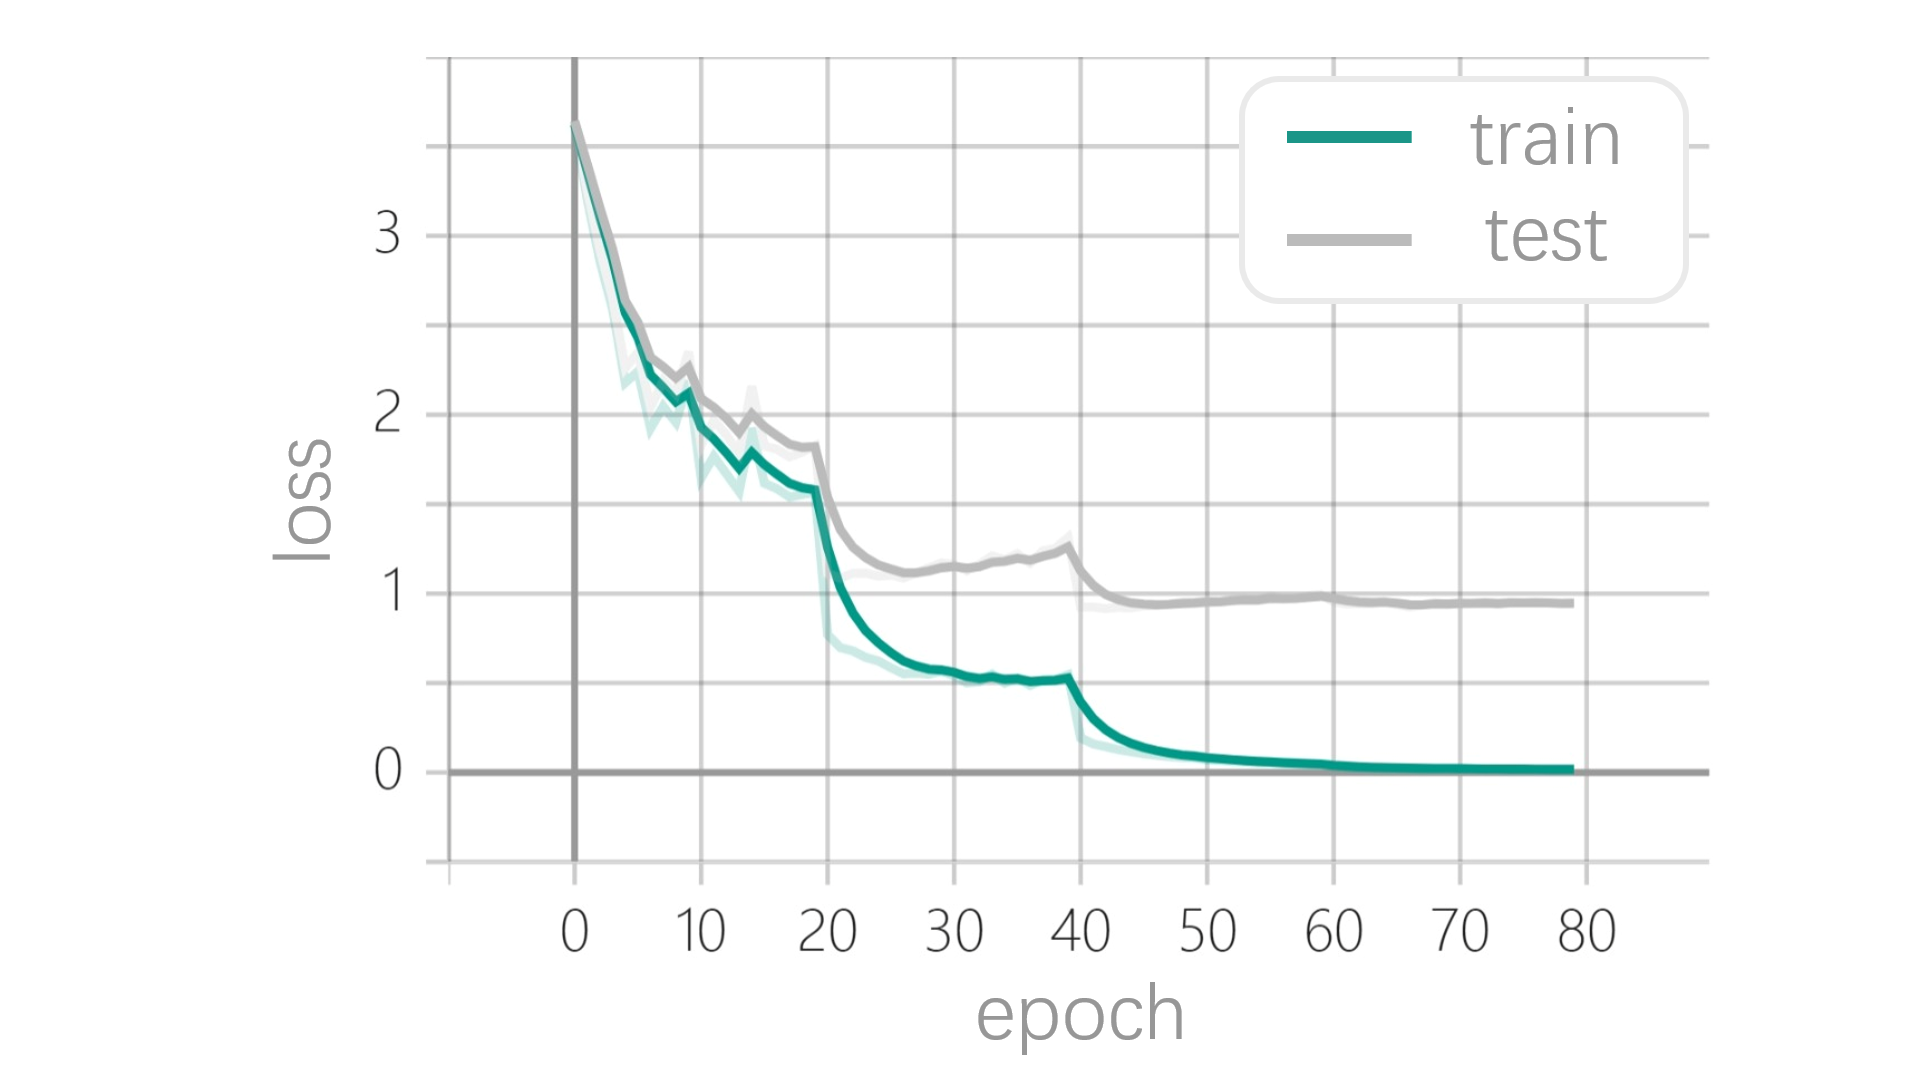
\includegraphics[width=\linewidth]
		{plot/ResNet/loss.png}
		\caption{ResNet loss}
	\end{subfigure}
	\begin{subfigure}{0.5\textwidth}
		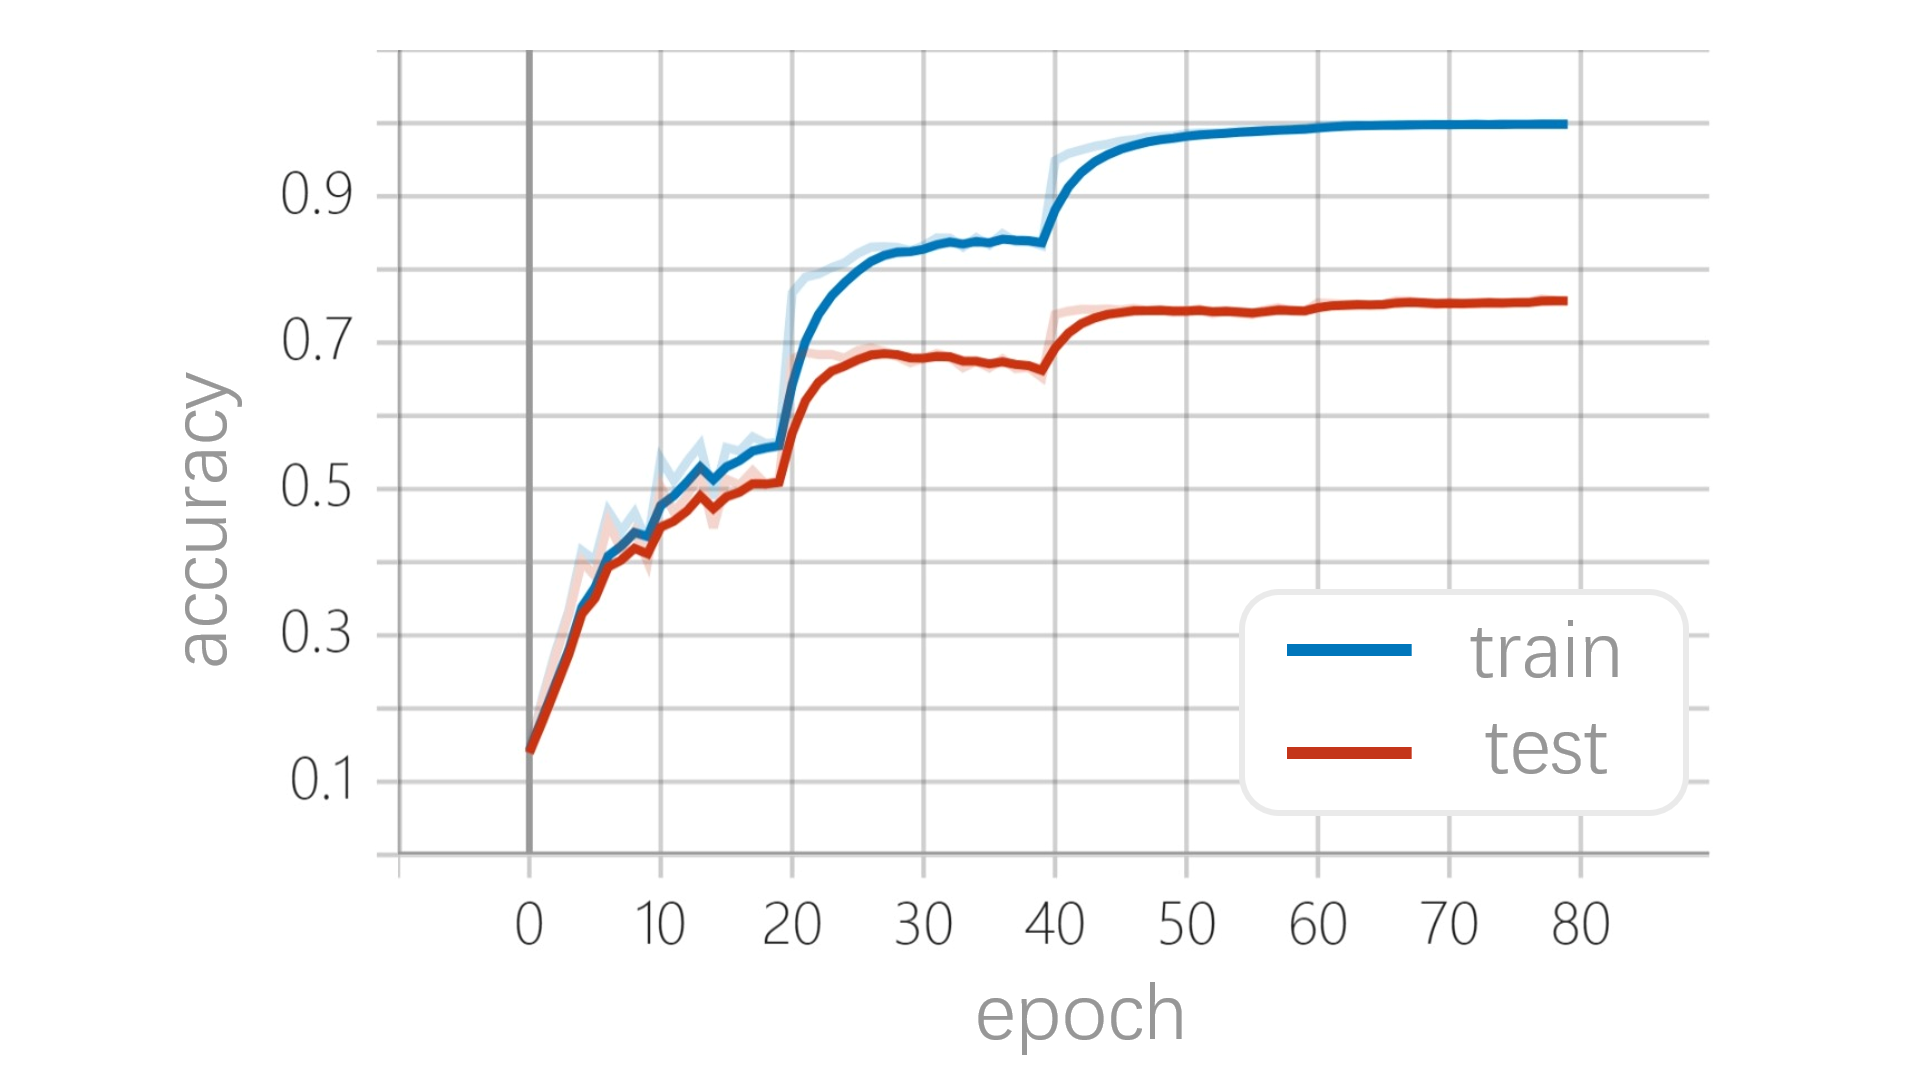
\includegraphics[width=\linewidth]
		{plot/ResNet/top1.png}
		\caption{ResNet accuracy}
	\end{subfigure}
	\caption{实验结果}
	\label{fig:Classify}
\end{figure}

\begin{table}[h]
	\centering
	\begin{tabular}{|l|c|c|c|c|} 
		\hline
		模型 
		& 训练集top1 & 训练集top5 
		& 测试集top1 & 测试集top5\\
		\hline
		ResNet & 0.99860 & 1.00000 & 0.75700 & 0.93120 \\
		ViT &  &  &  &  \\
		\hline
	\end{tabular}
	\caption{实验结果}
	\label{tab:Classify}
\end{table}
	
\end{document}